\documentclass[oribibl]{llncs}
\usepackage{llncsdoc}
\usepackage{multirow}
\usepackage{graphicx}
\graphicspath{{pics/}}
\usepackage[numbers,sort]{natbib}
\usepackage{amsmath}
\usepackage{subfigure}

\renewcommand{\refname}{References}  % for the article class
\renewcommand{\bibname}{References}  % for the report or book class

\begin{document}

\title{HOMI: Searching Higher Order Mutants For Software Improvement}

\author{Author(s)
%Fan Wu\inst{1}         \and
%		Mark Harman\inst{1}        \and
%		Yue Jia\inst{1}         \and
%		Jens Krinke\inst{1}
}


\institute{Institution(s) hidden for anonymity
%Department of Computer Science, UCL, Gower Street, London WC1E 6BT, UK \\
%              \email{\{fan.wu.12,mark.harman,yue.jia,j.krinke\}@ucl.ac.uk} 
}

\maketitle

\begin{abstract}

This paper introduces HOMI, a Higher Order Mutation based approach for Genetic Improvement of software,
%We propose using Higher Order Mutation for Genetic Improvement of software in this paper, 
in which the code modification granularity is finer than in previous work while scalability remains.
HOMI applies the NSGAII algorithm to search for higher order mutants that improve the non-functional properties of a program while passing all its regression tests.
%We use Higher Order Mutation to operate on the subjects at this finer granularity, while regression tests are used to maintain the functionality.
Experimental results on four real-world C programs shows
%A preliminary sensitivity analysis suggests 
that up to 14.7\% improvement on time or 19.7\% on memory are found using only First Order Mutants.
By combining these First Order Mutants, HOMI found Higher Order Mutants achieve up to 18.2\% improvement on the time performance.
A further manual analysis suggests that, 88\% of the mutation changes cannot be generated using line based `plastic surgery' Genetic Improvement approaches.
\end{abstract}

\section{Introduction}
\label{sec_intro}

Optimising software for better performance such as speed and memory consumption can be demanding, especially when the resources in the running environment are limited.
Manually optimising such non-functional properties while keeping or even improving the functional behaviour of a software is challenging. This becomes a even harder task if the properties considered are competing with each other~\cite{Harman:2012:GCC:2351676.2351678}. Search-Based Software Engineering (SBSE)~\cite{Harman2001833} has demonstrated many potential solutions, for example, speed up software systems \cite{5688317, Langdon:2014:IMI:2576768.2598244}, reduce memory consumption \cite{Wu:2015:DPO:2739480.2754648} and energy usage \cite{Bruce:2015:REC:2739480.2754752}.

%Search-Based Software Engineering (SBSE)~\cite{Harman2001833} considers this optimisation problem as a search problem that can be solved by search algorithms.

Previous studies have applied different search-based techniques to automate the optimisation process~\cite{arcuri-ssbse-2011, 6035728,Brake:2008:ADS:1370018.1370031,hutter2009paramils}. However, scalability of these approaches remains a challenge. To scale up and optimise real world programs, recent studies use a so-called `plastic surgery' Genetic Programming (GP) approach. To reduce the search space, it represents solutions as a list of edits to the subject program instead of the program itself~\cite{Bruce:2015:REC:2739480.2754752,geneticimprovementJP}.
Each sequence of edits consists of inserting, deleting a piece of code, or swapping pieces of code.
To ensure scalability, this approach usually modifies programs at the `line' level of granularity (the smallest atomic unit is a line of code). As a results, it is challenging for the `plastic surgery' to optimise subject program in finer granularity. 

%Wu et al. used Deep Parameter Tuning to fine tune programs, where some internal variables were exposed and optimised, with a prior sensitivity analysis on the subject programs to ensure scalability~\cite{Wu:2015:DPO:2739480.2754648}.
%However the approach follows a complicated process where redundancy may reside in the search space.
%In this paper, we propose a more efficient approach using Higher Order Mutants.

Mutation Testing~\cite{demillo1978hints,5487526} is an effective testing technique to test software. It automatically inserts artificial faults in the programs under test, to create a set of faulty programs that are called `mutants'. These mutants are used to assess the quality of tests, to provide testing criterion for generating new tests \cite{Harman:2011:SHO:2025113.2025144}, to fixing software bugs~\cite{6035728}. More recently they have also been suggested as a means to perform sensitivity analysis~\cite{Wu:2015:DPO:2739480.2754648} and to optimise software \cite{Jia:2015:GIU:2739482.2768417}.

We introduce the HOMI approach to improve non-functional properties of software while preserving the functionality. HOMI utilises search based higher order mutantion testing \cite{Harman:2014:AME:2642937.2643008} to effectively explore the search space of varying versions of a program. Like other previous GI work \cite{Langdon:2014:IMI:2576768.2598244, Bruce:2015:REC:2739480.2754752,geneticimprovementJP}, HOMI relies on high-quality regression tests to check the functionality of the program. Given a program $p$ and its regression tests $T$. HOMI generates two types of mutants that can be used for performance improvement. A \textbf{GI-FOM} is constructed by making a single syntactic change to $p$, which improves some non-functional properties of $p$ while passing all the regression tests $T$. Having the same characteristics as GI-FOMs, a \textbf{GI-HOM} is constructed from the combination of GI-FOMs.


%where mutants with a single fault are First Order Mutants (FOM) and those with more than one fault inserted are called Higher Order Mutants (HOM)~\cite{Harman:2011:SHO:2025113.2025144}.

By combining with Mutation Testing, we specifically utilise equivalent mutants which are expressly avoided by mutation testers where possible \cite{7194639}. 
%To reduce the search space, HOMI analyses the First Order Mutants (FOMs) to find those most sensitive to the property to be optimised. A subsequent multi-objective search algorithm is used for combinations of FOMs that have better runtime performance, but only mutate the most sensitive parts of the program.
%In this paper, we aim to search for Higher Order Mutants that improve the runtime performance but still preserve the functionality of the programs under optimisation~\cite{Jia:2015:GIU:2739482.2768417}.
%Therefore, by combining with Mutation Testing, we specifically utilise equivalent mutants which are expressly avoided by mutation testers where possible \cite{}.
%To reduce the search space, we analyse the First Order Mutants to find those most sensitive to the property to be optimised.
%A subsequent Genetic Algorithm searches for combinations of FOMs that have better runtime performance, but only mutate the most sensitive parts of the program.
%We also conduct a static analysis to show how many of the changes in the optimised HOMs cannot be achieved by patch-based approaches.
We implemented a prototype tool to realise the HOMI approach. The tool is designed to focus on two aspects of software runtime performance, execution time and memory consumption. Time and space are important qualities for many software, especially on portable devices or embedded systems where the runtime resources are limited. Moreover, these two qualities are usually competing with each other, yielding an interesting multi-objective solution space. Our tool produces a set of non-dominated GI-HOMs (thus forming a Pareto front). We evaluate our tool using four open source benchmarks. Since the tool requires no prior knowledge about the subjects, it can be easily applied to other programs.

The paper presents evidence that using Higher Order Mutation is an effective, easy to adopt way to improve existing programs. 
The experimental results suggest that equivalent FOMs can improve the subject programs by 14.7\% on execution time or 19.7\% on memory consumption.
Further results show that by searching for GI-HOMs, we can achieve up to 18.2\% time reduction on extreme cases.
Our static analysis suggests that 88\% of the changes in GI-HOMs cannot be achieved by `plastic surgery' based approaches.
The contributions of the paper are as follows:
\begin{enumerate}
\item We introduce an automatic approach to improve programs via Higher Order Mutation, which explore program search space at a fine granularity while maintaining good scalability.
%which is easy to adapt to other programs with different sizes.
\item We evaluate our approach on four open source programs with different sizes. We report the results and demonstrate that our approach is able to reduce the execution time by up to 18.2\% or to save the memory consumption by up to 19.7\%.
\item The results of a manual analysis are reported to show that our approach works on a smaller granularity such that 88\% of the changes found by our approach cannot be achieved by a line based `plastic surgery' approaches.
\item We also show evidence that it is possible to combine the HOMI approach with Deep-Parameter-optimisation approach to further improve the performance on four cases. 

\end{enumerate}

%The rest of the paper is organised as follows. 
%Section~\ref{sec_method} elaborates the approach we used in this paper.
%Section~\ref{sec_exp} gives details on the experimental settings.
%The results are reported in Section~\ref{sec_result}, followed by the discussion of threats to validity in Section~\ref{sec_threat}.
%Related works are summarised in Section~\ref{sec_related}, and we conclude in Section~\ref{sec_conclusion}.


%\section{Mutation Testing}
%\pagebreak

\section{The HOMI approach}
\label{sec_method}

We propose the HOMI approach, a higher order mutation based solution to GI. \figurename~\ref{fig_framework} shows the overall architecture of the HOMI approach. Given a subject program with a set of regression tests, and some optimisation goals, HOMI applies SBSE to evolve a set of GI-HOMs that improve the properties of interest while passing all the regression tests.  To explore the search space efficiently, we follow the current practice of GI in separating our approach into two stages \cite{6733370}. In the first stage, we apply first order mutation to find locations in the program at which making changes will lead to significant impact on the optimisation goals. In the second stage, we apply a multi-objective search algorithm at these program locations to construct a Pareto front of GI-HOMs. 

%Our approach can be divided into two steps: sensitivity analysis and searching for Higher Order Mutants.
%The whole process is illustrated in \figurename~\ref{fig_framework}.
%The approach takes the subject under optimisation, its test cases and the properties of interest as inputs.
%It first uses a mutation engine to generate the FOMs of the subject program, then evaluates them to collect sensitivity information.
%This process is detailed in Section~\ref{sec_sensitivity}.
%In the second step, it uses FOMs and sensitivity information to search for HOMs that have better time or memory performance than the original subject.
%The searching process is elaborated in Section~\ref{sec_hom}.
%We ask four Research Questions in Section~\ref{sec_rq}.

\vspace{-5mm}

\begin{figure}[h]
\centering
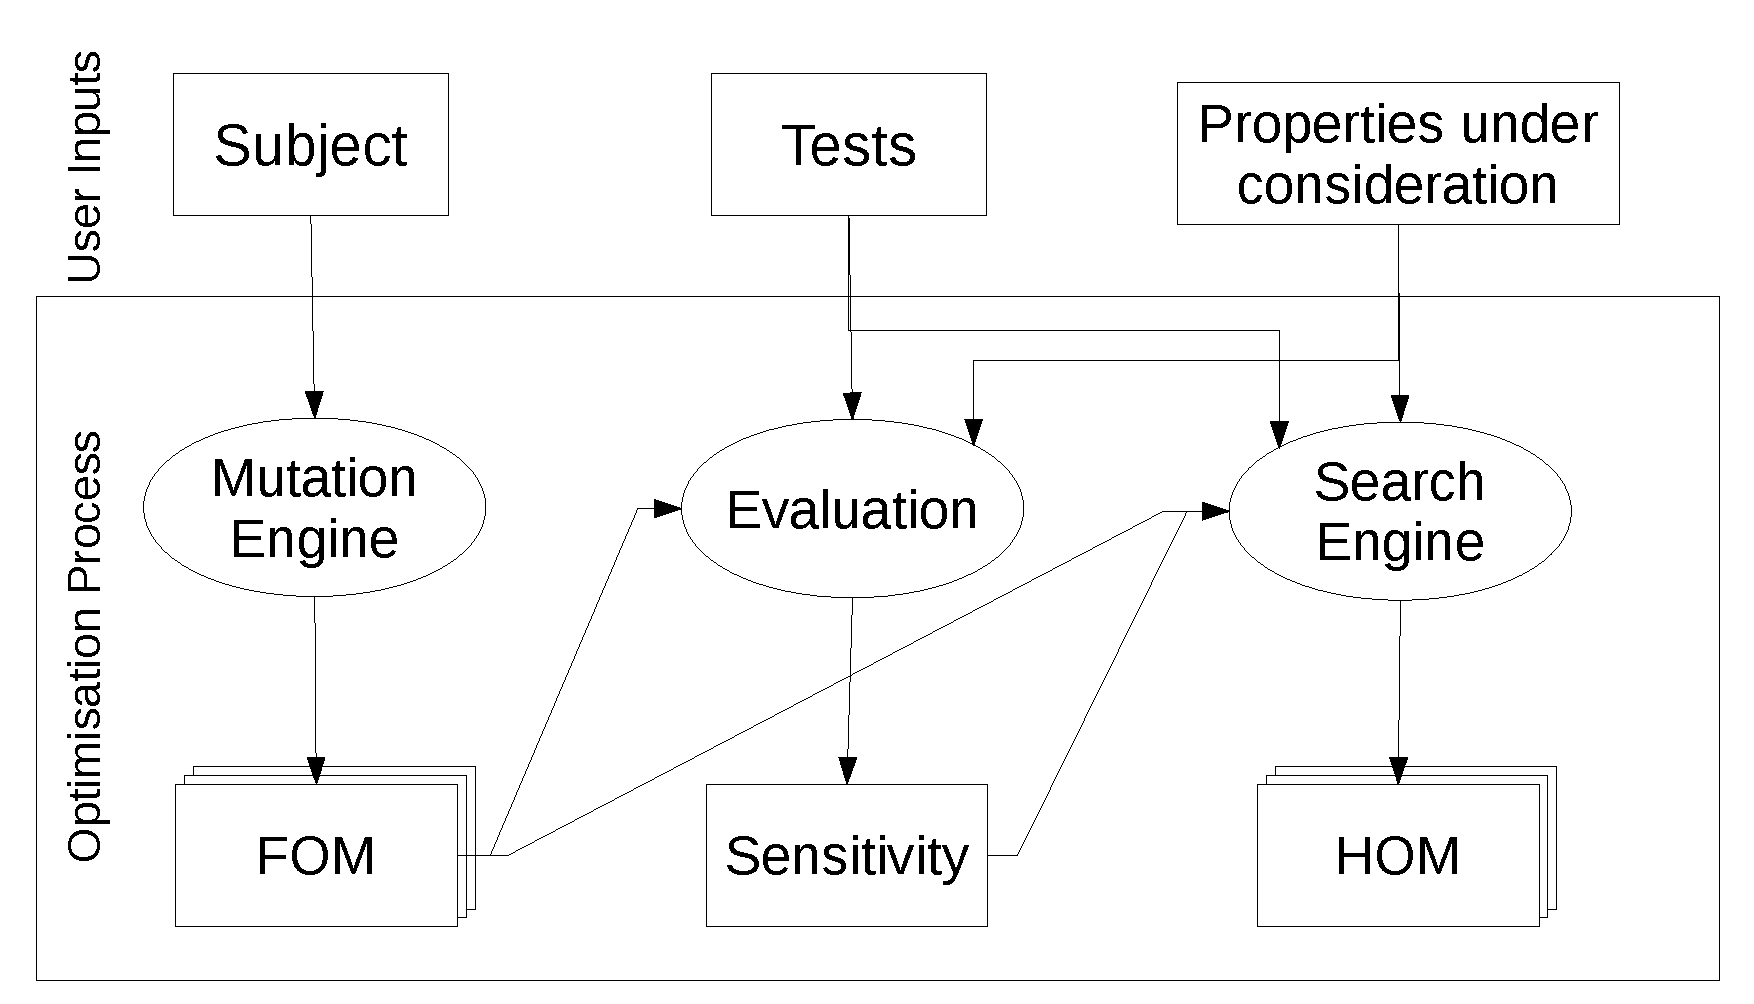
\includegraphics[width=1.0\textwidth]{framework}
\caption{The overall architecture of the HOMI approach.}\label{fig_framework}
%\caption{Framework of Higher Order Mutants searching. Given a subject under optimisation, it's tests and the runtime properties of interest, the optimisation process first conducts sensitivity analysis on FOMs, then use this information to search for HOMs with better performance.}
\end{figure}

\vspace{-7mm}

\subsection{Stage I: Sensitivity Analysis}
\label{sec_sensitivity}

Sensitivity analysis has been shown to be an effective way to reduce the search space in previous GI work~\cite{6733370,Bruce:2015:REC:2739480.2754752,6035728}. Given a subject program under optimisation, some code pieces may have a greater impact on the properties of interest than others. Sensitivity analysis seeks to find small portions of code that have the greatest impact on the properties of interest. Thus, the subsequent optimisation  can focus on a manageable amount of code, effectively reducing the search space. We use a first order mutation based sensitivity analysis approach to gather sensitivity information; this approach was introduced by Wu et al.~\cite{Wu:2015:DPO:2739480.2754648}. We use this form of sensitivity analysis because it provides finer granularity than traditional statement or line based sensitivity analysis.  


%% these will move to the background
%First Order Mutants were originally used for Mutation Testing~\cite{demillo1978hints}, a method of measuring the quality of test cases by inserting artificial faults.
%In Mutation Testing, a set of Mutation Operators is defined to mutate the subject program, each of which consists of a simple syntactic rule to change the subject program to generate mutants, such as changing the arithmetic operator `\texttt{+}' to `\texttt{-}'.
%Mutants generated by applying a Mutation Operator once to the original program are called First Order Mutants, while those generated from applying a Mutation Operator to a mutant are called Higher Order Mutants.
%We use FOMs for the sensitivity analysis because they by definition only differ from the original program in a syntactic change, therefore we can measure the sensitivity in a fine granularity.


As shown in \figurename~\ref{fig_framework}, HOMI first generates a set of FOMs of the subject program and then evaluates them using a fitness evaluation harness. The evaluation harness is composed of regression tests and the measurement components for optimisation goals. It runs each FOM on all the tests and outputs the measurements of the optimisation goals as fitness values.  After the fitness evaluation, HOMI removes FOMs that fail any regression tests and keeps only the survived ones. We do this because any mutants that pass all the regression tests are more likely to preserve the correctness of the subject. Finally, HOMI applies a non-dominated sorting~\cite{996017} to rank all the survived FOMs by their fitness values.
 
%To ensure the changes do not break the functionality, we use a regression test suite.
%A mutant is said to be `equivalent' with respect to a regression test suite if it passes all the regression tests.
%We discard all the mutants that are not equivalent to the original since we want to preserve the correctness of the subject.
%We gather the runtime performance of each equivalent mutant, that is time and memory consumption in this work.

The sensitivity analysis stage outputs a set of GI-FOMs. These FOMs are ``potentially equivalent mutants'' with respect to the regression test suites and have a positive impact on the properties of interest.  We measure the sensitivity of code based on the FOMs' fitness values.  A piece of code $A$ is said to be more sensitive than another piece $B$, if a FOM generated from $A$ dominates the FOM generated from $B$ on the Pareto front. The range of a code piece can be measured at different granularity levels by aggregating the results of FOMs, such as at the syntactic symbol, the statement level, or the nesting code block level. The GI-FOMs generated and their sensitive information are passed to the next search stage as inputs.



% I don't get this, but seems to much details.
%To avoid overlapping code pieces (meaning redundant search space), we define our code piece as a mutable symbol, which is a syntactic symbol to which a Mutation Operator can be applied.
%For instance, the arithmetic operator `\texttt{+}' is a mutable symbol since it can be mutated to other arithmetic operators.


\subsection{Stage II: Searching for GI-HOMs}
\label{sec_hom}

In the second stage, HOMI applies a multi-objective algorithm to search for a set of improved versions of the original program in the form of HOMs. We use an integer vector to represent HOMs, which is a commonly used data representation in search based Higher Order Mutation Testing \cite{Jia20091379}. Each integer value in the vector encodes whether a mutable symbol is mutated and how it is mutated. For example, given a mutant generated from the arithmetic operator `\texttt{+}',  a negative integer value means it is not mutated while the integer $0$, $1$, $2$, $3$ indicate that the code is mutated to `\texttt{-}', `\texttt{*}', `\texttt{/}', `\texttt{\%}' respectively.  In this way, each FOM is represented as a vector with only one non-negative number and HOMs can be easily constructed by the standard crossover and mutation search operators. 

%Therefore, combining these FOMs may generate HOMs that inherit the strengths of the FOMs that they are generated from, and yield better performance than any FOM alone.
%Selecting FOMs to form HOMs is a multi-objective search problem, thus we apply NSGA-II~\cite{996017} to search for HOMs with better performance.


The algorithm takes the GI-FOMs as input and repeatedly evolves HOMs that inherit the strengths of the GI-FOMs from which they are constructed and yield better performance than any GI-FOMs alone. The fitness function that guides the search is defined as the sum of the measurement of each optimisation property over a given test suite. Given a set of N optimisation goals, for each mutant $M$, the fitness function $f_n(M)$ for the nth optimisation goal is formulated as follow:

$$ Minimisation ~~~~f_n(M)=
\begin{cases}
    \sum C_i(M)      & \quad \text{if } M \text{ passes all test cases}\\
    C_{MAX}  & \quad \text{if } M \text{ fails any test case}\\
\end{cases}
$$

%The fitness function is sum by the measurement of the execution time and memory consumption over a given test suite.
%More formally, for each mutant $M$, the fitness of $M$ is formulated as:
%$$f(M)=
%\begin{cases}
%    (\sum t_i(M), \sum m_i(M))       & \quad \text{if } M \text{ passes all test cases}\\
%    (T_{MAX}, M_{MAX})  & \quad \text{if } M \text{ fails any test case}\\
%\end{cases}
%$$

The fitness function is a minimisation function where $C_i(M)$ is the measurement of the optimisation goal $n$ when executing the test $i$. If the mutant $M$ fails any regression tests, we consider it as a bad candidate and assign it with the worst fitness values $C_{MAX}$. The algorithm produces a Pareto front of GI-HOMs. Each HOM on the front represents a modified version of the original program that passes all the regression tests while no property of interest can be further improved without compromising at least one other optimising goal.

%
%where $t_i(M)$ is the time consumption of $M$ on the $i$th test case, and $m_i(M)$ is the `high-water mark' for virtual memory consumption.
%


\subsection{Implementation}
\vspace{-4mm}
We implemented a prototype tool to realise the HOMI approach. The HOMI tool is designed to optimise two non-functional properties (running time and memory consumption) for C programs.
In the fitness evaluation harness, we use \emph{Glibc}'s \emph{wait} system calls to gather the CPU time, and we instrument the memory management library to measure the `high-water' mark of the memory consumption. We choose to measure virtual instead of physical memory consumption because the physical memory consumption is non-deterministic. This means it depends on the workload of the machine. By contrast, the virtual memory used is always an upper bound of the physical memory actually used.

HOMI uses the open source C mutation testing tool, Milu \cite{JiaH08a} to generate mutants. We chose Milu because it features search based higher order mutation and can be used as an external mutant generator. By default, Milu supports only the traditional C mutation operators \cite{AgrawalDHHHKMMS89}. As memory consumption is one of the optimisation goals, we extended the original version of Milu to support Memory Mutation Operators proposed by Nanavati et al.~\cite{7107449}. \tablename~\ref{tab_mutationoperator} lists the Mutation Operators used in HOMI and their brief descriptions. During the search stage, HOMI transforms the internal integer vector representation of the candidate HOM to the data format recognisable by Milu, then invokes Milu to generate the HOM.
\vspace{-5mm}
\begin{table}[ht]
\caption{Mutation Operators used by HOMI}
\vspace{-6mm}
\label{tab_mutationoperator}
\begin{center}
\begin{tabular}{lll}
Category & Name    & Description                                          \\
\hline
\multirow{6}{*}{\begin{tabular}[c]{@{}l@{}}Selective\\ Mutation\\ Operators\end{tabular}} & ABS     & Change an expression \texttt{expr} to \texttt{ABS(expr)} or \texttt{-ABS(expr)} \\
& OAAN    & Change between \texttt{+}, \texttt{-}, \texttt{*}, \texttt{/}, \texttt{\%} \\
& OLLN    & Change between \texttt{\&\&}, \texttt{||} \\
& ORRN    & Change between \texttt{>}, \texttt{>=}, \texttt{<}, \texttt{<=}, \texttt{==} \\
& OIDO    & Change between \texttt{++}x, \texttt{{-}-}x, x\texttt{++}, x\texttt{{-}-} \\
& CRCR    & Change a constant \texttt{c} to \texttt{0}, \texttt{1}, \texttt{-1}, \texttt{c+1}, \texttt{c-1}, \texttt{c*2}, \texttt{c/2} \\
\hline
\multirow{9}{*}{\begin{tabular}[c]{@{}l@{}}Memory\\ Mutation\\ Operators\end{tabular}}    & REC2M   & Replace \texttt{malloc()} with \texttt{calloc()} \\
& RMNA    & Remove \texttt{NULL} assignment \\
& REDAWN  & Replace memory allocation calls to \texttt{NULL} \\
& REDAWZ  & Replace allocation size with \texttt{0} \\
& RESOTPE & Replace \texttt{sizeof(T)} with \texttt{sizeof(*T)} \\
& REMSOTP & Replace \texttt{sizeof(*T)} with \texttt{sizeof(T)} \\
& REM2A   & Replace \texttt{malloc()} with \texttt{alloca()} \\
& REC2A   & Replace \texttt{calloc()} with \texttt{alloca()} \\
& RMFS    & Remove \texttt{free()} statement \\
\hline
\end{tabular}
\end{center}
\end{table}
\vspace{-8mm}
%\tablename~\ref{tab_mutationoperator} lists the Mutation Operators we used in this work and their brief descriptions.
%They are divided into two groups: traditional Selective Mutation Operators and Memory Mutation Operators.
%We choose Selective Mutation Operators because they have been widely used in the recent mutation analysis experiments and they have been shown their high efficiency in covering most kinds of code changes~\cite{5487526}.
%Since we focus on both time and memory performance, more time/memory related Mutation Operators may provide additional potential of improvement.
%Therefore we include Memory Mutation Operators~\cite{7107449,Wu2016} that mainly mutate memory management calls, which have been shown to have great impact on both time and memory performance~\cite{Zorn:1992:EMS:142181.142200}.


%(** fan check search operator if correct)

The HOMI tool employs a customised NSGA-II~\cite{996017} to evolve GI-HOMs. During the search process, HOMI maintains a population of candidate HOMs. For each generation,  the uniform crossover and mutation are performed to parent HOMs, generating offspring HOMs that are later evaluated using the fitness functions mentioned. A tournament selection is then performed to form the next generation. This process is repeated until a given budget of evaluation times is reached. Finally HOMI will generate a set of non-dominating GI-HOMs that perform better than the original program on time and/or memory consumption.


\section{Empirical Study}
\label{sec_exp}

This section first discusses the research questions we address in our empirical evaluation of the HOMI tool, followed by an explanation of the chosen subjects, tests and experiment settings.

%In this section, we provide more details regarding the experimental settings.
%The Mutation tool and the summary of the subject programs can be found in Section~\ref{sec_milu} and Section~\ref{sec_subject} respectively.
%Section~\ref{sec_preprocessing} describes some techniques used to reduce the search space.
%Other experimental settings can be found in Section~\ref{sec_searchsetting}.



\subsection{Research Questions}
\label{sec_rq}


Since the HOMI approach generates GI-HOMs from the combination of FOMs, a natural first question to ask is `whether existing FOMs can be used to improve software'.  This motivates our first research question. 

\vspace{2mm}
\noindent\textbf{RQ1: Can GI-FOMs improve program performance while passing all of its regression tests?}
\vspace{2mm}

To answer this question, we run HOMI for sensitivity analysis only and report how much running time and memory can be saved by GI-FOMs. Of course, the answer also depends on the quality of the regression tests. All the tests used in our evaluation are regression tests generated by developers for real world systems. However, they may still not be sufficient to reveal the faults introduced by mutation. To make our experiment more rigorous, we carried out a pre-analysis in our evaluation. We analyse the function coverage of each subject using the GNU application \emph{Gcov} and HOMI is set only to mutate the functions that are covered by regression tests. 


\vspace{2mm}
\noindent\textbf{RQ2: How much improvement can be achieved by GI-HOM in comparison with GI-FOMs?}
\vspace{2mm}

If GI-FOMs alone can improve performance, we expect that GI-HOMs will inherit some strengths from the GI-FOMs and improve the performance further. To answer this question, we use HOMI to generate a GI-HOM Pareto front and investigate whether the GI-FOM solutions generated are on the Pareto front. Furthermore, it is interesting to see whether the new memory mutation operators help to improve the performance. This motivates our sub-question which studies the effect on mutation operators used. 

\vspace{2mm}
\noindent\textbf{RQ 2.1 How does the improvement achieved by applying the traditional mutation operators only compare to applying both of the traditional and memory mutation operators? }
\vspace{2mm}

We answer this question by comparing the HyperVolume quality indicator of the Pareto fronts generated from HOMI using both sets of mutation operators. Given a Pareto front A and a reference Pareto front R, HyperVolume is the volume of objective space dominated by solutions in A. To take into account the stochastic nature of the search algorithms, we repeat both experiments 30 times. We use the non-parametric Wilcoxon-signed rank tests to assess the statistical significance of the HyperVolume and Vargha-Delaney effect size to further assess the magnitude of the differences \cite{STVR:STVR1486, Neumann2015}. 

\vspace{2mm}
\noindent\textbf{RQ3: Can `plastic surgery' GP based GI approach find edit sequences to construct the GI-HOMs found by HOMI?}
\vspace{2mm}

We ask this question because we want to understand whether the granularity of mutation changes can be produced by the  `plastic surgery' GP approach. The  `plastic surgery' GP approach is a popular GI approach which searches for a list of edits from the existing source code. Typical changes generated by the GP approach are movements or replacements of different lines of code \cite{justyna2013, 6733370}. To answer this question, we carried out a sanity-check experiment manually using all the GI-HOMs found. For each GI-HOM, we search the entire program to see if the mutated statement exists in the program. If it does, the GI-HOM can be constructed by the patches generated from the GP approach easily. Otherwise, we consider the line/statement based `plastic surgery' GP might not able to generate the GI-HOM directly. 

\vspace{2mm}
\noindent\textbf{RQ4 Can HOMI be combined with Deep Parameter Optimisation to achieve further improvement?}
\vspace{2mm}

Finally, we want to investigate whether the HOMI approach can be combined with other types of GI techniques. Deep Parameter Optimisation is one of the state-of-the-art parameter tuning based GI techniques. It seeks to optimise library code used instead of the source code of the subjects \cite{Wu:2015:DPO:2739480.2754648}. We have contacted the authors of the Deep Parameter Optimisation work to provide a set of memory allocation libraries that were optimised for the time and memory performance for each subject. We answer this research question by evaluating the GI-HOMs after linking them to Deep-Parameter-optimised libraries, then comparing them with their performance before the linking, and with the performance of the original program after linking to Deep-Parameter-optimised libraries.




%
%
%\begin{enumerate}
%\item[\textbf{RQ1}] Can First Order Mutants improve performance while maintaining functionality?
%\end{enumerate}
%
%We ask the first question as the baseline and motivation of this work.
%If we find that some First Order Mutants alone have better performance than the original program, it would be interesting to search for combinations of FOMs that inherit the strengths of the FOMs.
%On the other hand, if there is no FOM that outperforms the original, it would still be interesting to see whether there is synergy between FOMs such that they form HOMs that performs better than any of the FOMs alone and the original.
%We answer this question by generating and evaluating FOMs, and comparing their runtime performance with the original programs.
%
%\begin{enumerate}
%\item[\textbf{RQ2}] How much improvement can be achieved in Higher Order Mutants, comparing with the original and FOMs?
%\begin{enumerate}
%\item[\textbf{RQ2.1}] How much improvement can be achieved by using traditional Mutation Operators alone?
%\item[\textbf{RQ2.2}] How much improvement is accounted for by adding Memory Mutation Operators?
%\end{enumerate}
%\end{enumerate}
%
%After evaluating FOMs, we are interested in searching for better performance in HOMs.
%By applying search algorithms, we expect some HOMs that inherit some or all of the strengths from the FOMs they are formed from.
%We ask the second research question to understand the optimal performance we can achieve by combining FOMs.
%Furthermore, it is interesting to see whether the Memory Mutation Operators help improving the performance.
%Therefore, we ask two sub-questions to understand how much improvement can be achieved by using traditional Mutation Operators alone, and how much additional improvement can be achieved by adding Memory Mutation Operators.
%We answer these questions by applying search algorithm on traditional mutants alone, and on traditional mutants and memory mutants together, to see the improvement respectively.
%
%\begin{enumerate}
%\item[\textbf{RQ3}] How many of the changes in improved HOMs cannot be generated by patch-based approaches?
%\end{enumerate}
%
%We ask the third research question because we want to understand whether increasing the granularity of code changes provides more improvement potential, compared to patch-based GI.
%If there are mutational changes that cannot be achieved by patching, then it is likely that some improvement may never be found by patch-based approaches, thus finer granularity may help in finding better performance.
%We answer this question by conducting a static analysis on the source code of the subjects to see whether the mutational changes can be generated from other code pieces in the program.
%
%\begin{enumerate}
%\item[\textbf{RQ4}] Do Deep-Parameter-optimised library provide further improvement?
%\end{enumerate}
%
%Deep Parameter Optimisation is a recently proposed technique that optimises the library code instead of the source code of the subjects~\cite{Wu:2015:DPO:2739480.2754648}.
%It also focused on the time and memory performance of the subjects.
%Therefore it is interesting to see how the improvement changes when we link HOM-optimised subjects with Deep-Parameter-optimised libraries.
%We answer this research question by evaluating the optimised HOMs after linking them to Deep-Parameter-optimised libraries, then comparing them with their performance before the linking, and with the performance of the original program after linking to Deep-Parameter-optimised libraries.





\subsection{Subject programs and tests}
\label{sec_subject}

We optimise four subjects in our proof-of-concept evaluation. 
\tablename~\ref{tab_subject} lists the subjects and their brief description. All tests used are regression tests, deemed to be useful and practical by their developers.
\emph{Espresso} is a fast application for simplifying complex digital electronic gate circuits.
\emph{Gawk} is the GNU \emph{awk} implementation for string processing.
\emph{Flex} is a tool for generating scanners, programs which recognise lexical patterns in text, and \emph{sed} is an editor that automatically modifies files given a set of rules. 
We use the \emph{espresso} version as well as its test cases from \emph{DieHard} project~\cite{Berger:2006:DPM:1133981.1134000}.
Version 4.1.0 of \emph{gawk} is used in this work.
The source code and the test cases can be found in the GNU archives.
We obtain the last two programs and corresponding test suites from the SIR repository~\cite{SIR2005}. 



\begin{table}[!ht]
\centering
\caption{Subject programs}
\label{tab_subject}
%\resizebox{0.5\textwidth}{!}{
\begin{tabular}{crrl}
\hline
Name & LoC & \# of Tests & Description \\
\hline
\emph{espresso} & 13,256 & 19 & Digital circuit simplification\\
%\hline
\emph{gawk} & 45,241 & 334 & String processing\\
%\hline
\emph{flex} & 9,597 & 62 & Fast lexical analyzer generator\\
%\hline
\emph{sed} & 5,720 & 362 & Special file editor\\
\hline
\end{tabular}%}
\end{table}




%\subsection{Preprocessing}
%\label{sec_preprocessing}
%
%In order to minimise the computation in the experiments, preprocessing is conducted before each of the two steps of the experiments.
%Before any FOM is generated, we first analyse the function coverage of each subject using the GNU application \emph{Gcov}.
%We only mutate the functions that have non-zero coverage, since a zero-coverage function is never executed, therefore mutating it will never affect the subject program.


\vspace{-3mm}
\subsection{Search Settings}
\label{sec_searchsetting}


In the sensitivity analysis stage, we pick the top 10\% most sensitive locations of GI-FOMs and only search for GI-HOMs from these locations. We use a relative ratio instead of an absolute number because the search space can be fairly adapted to the size of the subject. The choice of 10\% is based on our observation that the locations in the first 10\% are usually much more sensitive than the remaining locations since sensitivity seems to follow a power law, according to our informal observation. However, the ratio can be easily adapted as a parameter to our approach accordingly.


We repeat all HOMI experiments 30 times to cope with the non-deterministic nature of NSGAII. The NSGAII performs a tournament selection of size 2 and uniform crossover with a probability of 0.8. There are 50 HOMs in each generation and the algorithm stops at 100th generation. These numbers were chosen after initial calibration experimentation to determine suitable parameters for our search process. All of the experiments are carried out on a desktop machine with a quad-core CPU and 7.7 GB RAM running 64-bit Ubuntu version 14.04.


%
%After collecting sensitivity information, there could be thousands of mutable locations in a subject, yielding an extremely large solution space.
%Therefore we pick the top 10\% most sensitive locations and only search for HOMs generated from mutating them, in which case spaces needed to store the vector representations of HOMs are reduced, as well as the search space.
%We use a relative ratio instead of an absolute number to pick sensitive locations so that the search space is fairly adapted to the size of the subject, and 10\% is based on our observation that the locations in the first 10\% are usually much more sensitive than the remaining locations since sensitivity seems to follow a power law, according to our informal observation.
%However, the ratio can be easily adapted as a parameter to our approach accordingly.
%
%
%In the experiments, NSGA-II~\cite{996017} is used to search for HOMs.
%Tournament selection of size 2 and uniform crossover with a probability of 0.8 are performed in each generation.
%There are 50 HOMs in each generation and the algorithm stops at 100th generation.
%These numbers were chosen after a few trial runs to make sure the results are stable.
%
%
%
%In regards of fitness function, \emph{Glibc}'s \emph{wait} system calls are used to gather the CPU time, and we instrument the memory management library to measure the high-water mark of the memory consumption.
%The search process was repeated 30 times to cope with the non-deterministic nature of Genetic Algorithm, and to perform influential statistical tests~\cite{STVR:STVR1486, Neumann2015}.
%All of the experiments are carried out on a desktop machine with a quad-core CPU and 7.7 GB RAM running 64-bit Ubuntu version 14.04.


\section{Results and Discussion}
\label{sec_result}

\newcommand{\homss}{GI-HOMs-Sel}
\newcommand{\homsa}{GI-HOMs-All}

%In this section, we present the experiment results and answer the Research Questions one in each subsection.

\subsection{Improvement by GI-FOMs}
\label{sec_resfom}

We begin by looking at the time and memory performance of the GI-FOMs generated from the sensitivity analysis stage to answer the RQ1. We calculated the improvement of GI-FOMs relative to the original program, and reported them in Column 2 and 5 in \tablename~\ref{tab_fomhom}. These measures are averaged from 10 repeated runs. By applying selective and memory mutation operators to generate FOMs, we found the improved versions of all four subjects, both on time and memory performance. More specifically, the improvement ranges from 0.9\% to 14.7\% on time and from 0.5\% to 19.7\% on memory performance.  
However, there might be a large gap between the memory and time improvement for some subject, for example, the GI-FOM of \emph{sed} can run up to  14.7\%  faster to only save 0.5\% memory. We conclude that even with the simplest changes introduced by first order mutation, the HOMI approach is able to improve the execution time and memory consumption. 

%Firstly, we evaluated the time and memory performance of those FOMs used for sensitivity analysis to answer the baseline question.
%The improvement of FOMs relative to the original is reported in Column 2 and 5 in \tablename~\ref{tab_fomhom}.
%By applying Selective and Memory Mutation Operators to generate FOMs, we find improvement on all four subjects, both on time and memory performance.
%More specifically, the execution time can be improved by up to 14.7\% (on \emph{sed}) and the improvement is up to 19.7\% on memory consumption (on \emph{flex}).
%Therefore, the answer to RQ1 is, yes, FOMs alone can improve programs, with the improvement ranging from 0.9\% to 14.7\% on time and from 0.5\% to 19.7\% on memory performance.


\subsection{Improvement by GI-HOMs}
\label{sec_reshom}

We now turn to the improvement found by GI-HOMs. Since improvement was found on GI-FOMs, it is interesting to investigate whether we can improve the performance further by combining them to form GI-HOMs. We applied NSGA-II~\cite{996017} to search for better performance in HOMs using Selective Mutation Operators (\homss{}) and using both Selective and Memory Mutation Operators (\homsa{}) respectively. Each experiment was repeated for 30 times and the best time/memory performance found for each subject is reported in \tablename~\ref{tab_fomhom}. 

%Since improvement were found on FOMs, it is interesting to investigate whether we can improve the performance further by combining FOMs to form HOMs.
%We applied NSGA-II~\cite{996017} to search for better performance in HOMs using Selective Mutation Operators (\homss{}) and using both Selective and Memory Mutation Operators (\homsa{}) respectively.
%Each Experiment was repeated for 30 times and the best time/memory performance found for each subject is reported in \tablename~\ref{tab_fomhom}.

\begin{table}[!ht]
\centering
\caption{Improvement on time and memory by GI-FOMs and GI-HOMs. \homss{} are found using only Selective Mutation Operators while \homsa{} and GI-FOMs are found using both Selective and Memory Mutation Operators}
\label{tab_fomhom}
\begin{tabular}{lrrr|rrr}
\hline
         &      & \multicolumn{1}{c}{Time (\%)} &               &               & \multicolumn{1}{c}{Memory (\%)} &               \\
Subject  & GI-FOMs & \homss{}         & \homsa{}          & GI-FOMs          & \homss{}           & \homsa{}          \\
\hline
\emph{espresso} & 5.2  & 6.5                      & \textbf{6.9}  & 1.6           & \textbf{1.7}               & \textbf{1.7}  \\
\emph{gawk}     & 2.3  & 6.7                      & \textbf{9.8}  & 2.5           & 1.9                        & \textbf{4.3}  \\
\emph{flex}     & 0.9  & \textbf{2.3}             & \textbf{2.3}  & \textbf{19.7} & \textbf{19.7}              & \textbf{19.7} \\
\emph{sed}      & 14.7 & \textbf{18.2}            & \textbf{18.2} & \textbf{0.5}  & \textbf{0.5}               & \textbf{0.5} \\
\hline
\end{tabular}
\vspace{-4mm}
\end{table}


The results of \homss{} are reported in Column 3 and 6, and those of \homsa{} are reported in Column 4 and 7. We immediately observe that GI-HOMs achieve greater improvement than GI-FOMs on execution time for all subjects, also on memory consumption for two out of four subjects. The greatest time improvement found by GI-HOMs can be promoted to 18.2\%, while the improvement can be up to four times better (on \emph{gawk}) than the improvement yielded from GI-FOMs. We also observe one case {\emph{gawk}), on which the \homss{} achieve less memory improvement compared with GI-FOMs, because they are lack of some memory-related changes that can only be achieved by Memory Mutation Operators. 

%By searching HOMs, the greatest time improvement can be promoted to 18.2\%, while the improvement can be up to four times of the improvement provided by FOMs.
%%In all but two cases (memory performance on \emph{flex} and \emph{sed}), better performance was found in HOMs than the best FOMs.
%Furthermore, in three cases (time performance on \emph{espresso} and \emph{gawk}, memory performance on \emph{gawk}), including Memory Mutation Operators provides further improvement, compared with those using Selective Mutation Operators only.



We combine the results of 30 runs for each experiment and plot the Pareto Fronts of GI-HOMs using all Mutation Operators, GI-HOMs using Selective Mutation Operators and GI-FOMs in \figurename~\ref{fig_pareto}.
In the figure, time (x-axis) and memory (y-axis) are both normalised to the original performance.
%FOMs are plotted in yellow triangles, HOMs using Selective Mutation %Operators only are represented by red squares and HOMs using all %Mutation Operators are represented by blue circles.
On all four subjects, we can see there is always an improvement from GI-FOMs to GI-HOMs, while the differences between \homss{} and \homsa{} are less clear. 
%Furthermore, there is an improvement when Memory Mutation Operators %are included on subject \emph{espresso} and \emph{gawk}, while %there is not much difference between these Pareto Fronts on the other %subjects.
To statistically demonstrate the difference, we calculated the HyperVolume~\cite{797969} of the Pareto Front of GI-HOMs using all Mutation Operators and those using Selective Mutation Operators over 30 runs, and applied Mann-Whitney-Wilcoxon \emph{U}-test on the HyperVolume. For subject \emph{espresso} and \emph{gawk}, the difference between HOMs (all) and HOMs (Selective) are significant ($p<0.01$) with a large effect size ($A_{12} > 0.9$), while for the other two subjects, the difference is not significant.

\begin{figure}[ht]
	\centering
	\subfigure[espresso]{
		\label{fig_pareto_espresso}
		\scalebox{1}{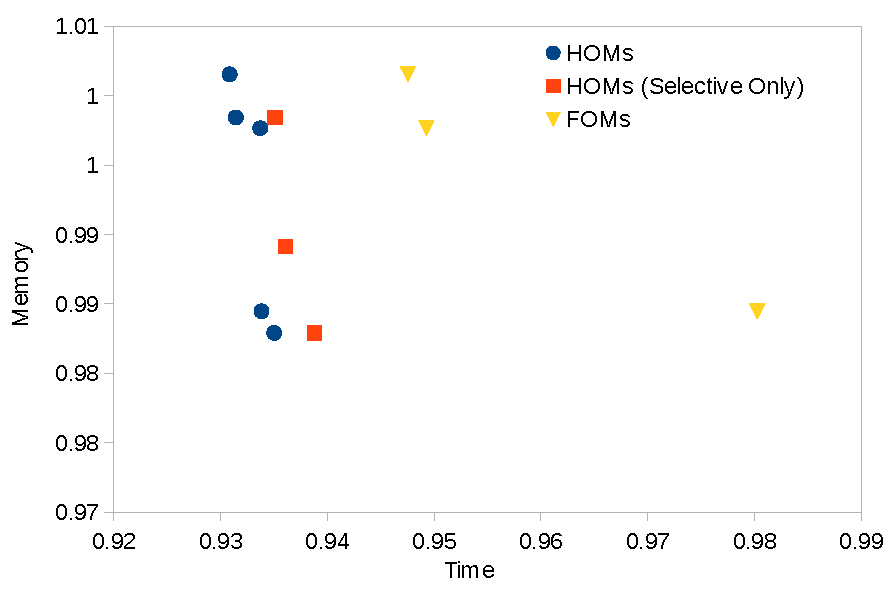
\includegraphics[width=0.47\textwidth]{pareto_espresso}}
	}
	\subfigure[gawk]{
		\label{fig_pareto_gawk}
		\scalebox{1}{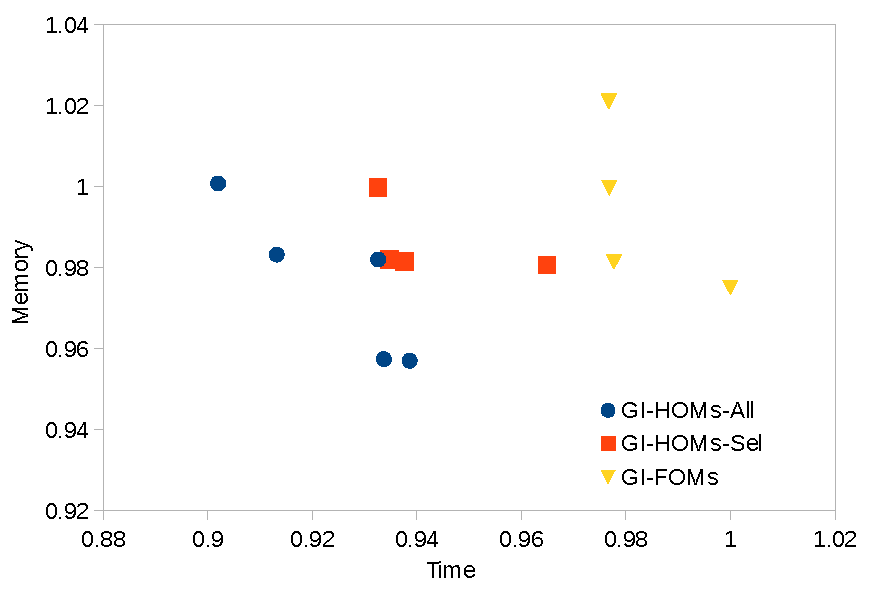
\includegraphics[width=0.47\textwidth]{pareto_gawk}}
	}
	\subfigure[flex]{
		\label{fig_pareto_flex}
		\scalebox{1}{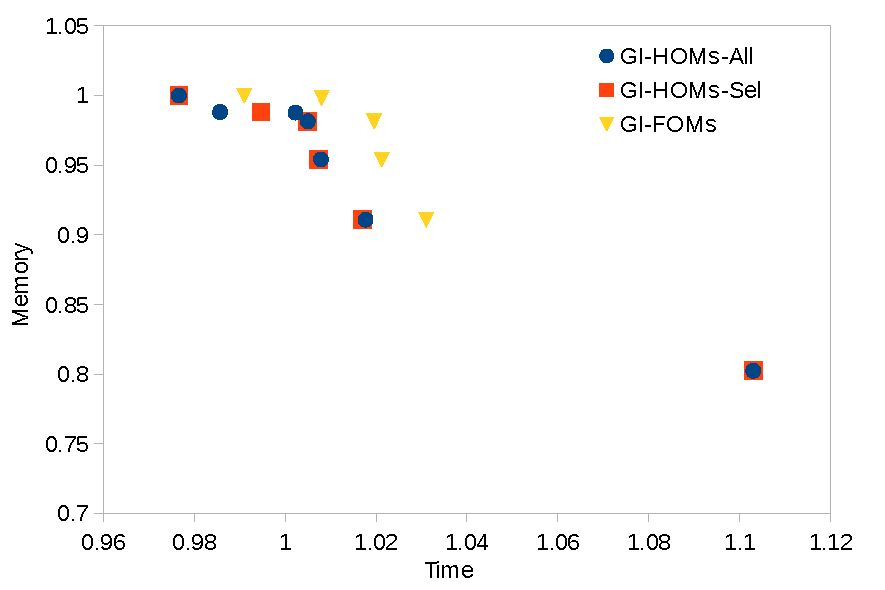
\includegraphics[width=0.47\textwidth]{pareto_flex}}
	}
	\subfigure[sed]{
		\label{fig_pareto_sed}
		\scalebox{1}{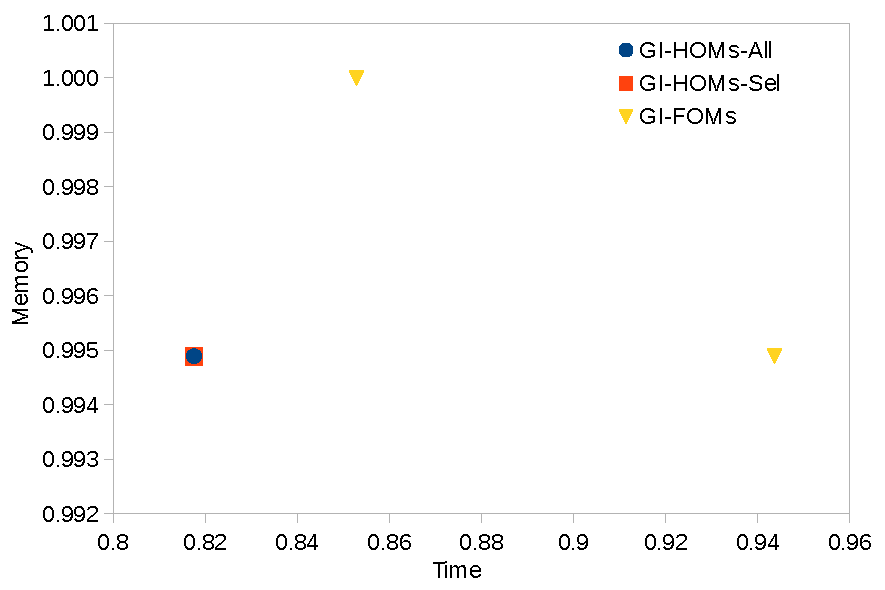
\includegraphics[width=0.47\textwidth]{pareto_sed}}
	}
	\vspace{-1em}
	\caption{Pareto Fronts of GI-HOMs and GI-FOMs for each subject. Lower and lefthand solutions dominate high and righthand solutions.}\label{fig_pareto}
\end{figure}

In summary, the answer to RQ2 is that GI-HOMs can improve the time performance by up to 18.2\% or the memory performance by up to 19.7\%. For the GI-HOMs using Selective Mutation Operators only, we found the same upper bound of the improvement, but only achieved sub-optimal solutions on two subjects.
By including Memory Mutation Operators, further improvement on these subjects were found.
Therefore, we can conclude that Memory Mutation Operators provide further improvement potentials for both time and memory optimisation.

\subsection{HOMI vs `plastic surgery' GP based GI}
\label{sec_resstatic}


This RQ investigates whether the granularity of mutation changes can also be generated by the `plastic surgery' GP approach. To answer this question, we investigated the GI-HOMs found in all experiments and manually reproduce them following the evolution rules used in the line/statement based `plastic surgery' GP approach \cite{justyna2013, 6733370}. All together HOMI found  273 mutations in the improved GI-HOMs across all subjects. We first applied a simple hill-climbing algorithm to clean up the mutations that do not contribute to the improvement. This step narrowed the number of mutations down to 141. %We then manually examined these mutations, and filtered out are in total 108 unique mutation changes.  (the same mutations may be found in several GI-HOMs).
In total, there are 108 unique mutations identified (the same mutations may be found in several GI-HOMs).

For each of the unique mutation changes, we search the entire program to see if the mutated line/statement exists in the program.  Because the typical changes generated by the `plastic surgery' GP approach are movements or replacements of different lines of code \cite{justyna2013, 6733370}, if a mutation does not appear somewhere else in the original source code, it cannot be generated directly from this form of GP approaches. The result shows that 95 (88\%) out of 108 mutations cannot be found in the original source code. Therefore, the answer to RQ3 is, there are 108 unique mutational changes found in the GI-HOMs, 88\% of which cannot be generated from the line based `plastic surgery' GP approach directly.

%To investigate whether those mutational changes can be generated from patch-based approaches, we investigated the mutants non-dominated by any other mutants in all experiments, and searched for their mutational changes in the original source code.
%We found there are 273 mutations among those mutants across all subjects.
%By appling a simple hill-climbing to clean up the mutations that do not contribute to the improvement, we narrowed down to 141 mutations.
%Among these mutations, there are in total 108 unique mutations (the same mutations may be found in several mutants).
%We then searched for these unique mutations in the original source code in the statement level.
%If a mutation does not appear somewhere else in the original source code, it cannot be generated from patch-based approaches since these approaches use the original source code as their code base to generate patches.
%The result shows that 95 (88\%) out of 108 mutations cannot be found in the original source code.
%Therefore, the answer to RQ3 is, there are 108 unique mutational changes in the improved HOMs, 88\% of which cannot be generated from patch-based approaches.

\subsection{HOMI combines with Deep Parameter Optimisation}
\label{sec_resdeep}

In the last Research Question, we want to understand whether the improvement can be preserved or even promoted if we combine GI-HOMs with Deep-Parameter-optimised memory management library. 
To answer this question, we contacted the authors of the Deep Parameter Optimisation work to obtain a set of memory allocation libraries that were optimised for the time and memory performance for each subject. We created four new optimised version of each subject by linking the most time/memory-saving GI-HOMs and libraries in pairwise.



The results are reported in \tablename~\ref{tab_deep}.
In the table, rows represent HOMI-improved programs and columns represent Deep-Parameter-optimised libraries, where `Original' indicates the original program or library, `T' indicates it is the most time-saving ones and 'M' indicates the most memory-saving ones.
All of the numbers are the improvement in percentage compared with the original version.
%specially, the combination of original program and original library is always 0\% improvement on either performance.
If in a combination (that does not involve the Original program/library), the time/memory performance is not worse than that of any of the `ingredient' program/library, it is highlighted in the bold font.
On the other hand, all the underlined performance are the ones that are worse than both of the `ingredient' program and library.
For subject \emph{sed}, there is only one GI-HOM on the Pareto Front, thus it is both the most time and memory-saving program.

% choose one table from:
\vspace{-4mm}
\begin{table}[ht]
\centering
\caption{HOMI combines with Deep Parameter Optimisation. Each cell reports the time improvement followed by memory improvement in percentage. `T' or `M' indicates it is most time-saving or memory-saving GI-HOM/optimised library.}
\label{tab_deep}
\resizebox{\textwidth}{!}{
\begin{tabular}{llrrr|llrrr}
\hline
                          &          & \multicolumn{3}{r|}{Memory Management Library} &                       &          & \multicolumn{3}{r}{Memory Management Library} \\
                          &          & Original       & Deep(T)       & Deep(M)      &                       &          & Original      & Deep(T)        & Deep(M)      \\
\hline
\multirow{3}{*}{\rotatebox[origin=c]{90}{\emph{espresso}}} & Original & 0/0            & 0.8/0.1       & 0.7/0.2      & \multirow{3}{*}{\rotatebox[origin=c]{90}{\emph{gawk}}} & Original & 0/0           & 5.4/1.6        & -0.2/2.3     \\
                          & GI-HOM(T)   & 6.9/-0.2       & 4.8/\textbf{0.1}       & 4.7/\textbf{0.2}      &                       & GI-HOM(T)   & 9.8/-0.1      & 5.6/\textbf{1.6}        & 5.4/\textbf{2.3}      \\
                          & GI-HOM(M)   & 6.5/1.7        & 4.7/\textbf{1.8}       & \textbf{6.7}/\textbf{1.7}      &                       & GI-HOM(M)   & 6.1/4.3       & \underline{4.1}/\textbf{5.8}        & 4.8/\textbf{5.5}      \\
\hline
\multirow{3}{*}{\rotatebox[origin=c]{90}{\emph{flex}}}     & Original & 0/0            & 15.7/-2.6     & -1.1/0.6     & \multirow{3}{*}{\rotatebox[origin=c]{90}{\emph{sed}}}  & Original & 0/0           & 7.9/-1208      & 5.6/2.0      \\
                          & GI-HOM(T)   & 2.3/0          & 14.4/-2.6     & -Inf/-Inf    &                       & GI-HOM(TM)   & 18.2/0.5      & \underline{5.8}/-1208      & \underline{4.1}/0.9      \\
                          & GI-HOM(M)   & -10.3/19.7     & -3.5/\textbf{19.7}     & -Inf/-Inf    &                       &    &             &              &           \\
\hline
\end{tabular}
}
\end{table}
\vspace{-4mm}

%\begin{table}[ht]
%\centering
%\caption{Best Improvement for each subject, using HOMs or Deep-Parameter-Optimisation approach. All numbers are normalised improvement to original subjects.}
%\label{tab_compare_deep}
%\resizebox{\textwidth}{!}{
%\begin{tabular}{llrr|rr}
%\hline
%         &          & \multicolumn{2}{c|}{Most Time-saving}       & \multicolumn{2}{c}{Most Memory-saving}      \\
%Subject  & Approach & Time Reduction (\%) & Memory Reduction (\%) & Time Reduction (\%) & Memory Reduction (\%) \\
%\hline
%espresso & HOMs     & 6.9                 & -0.2                  & 6.5                 & 1.7                   \\
%         & Deep     & 0.8                 & 0.1                   & 0.7                 & 0.2                   \\
%\hline
%gawk     & HOMs     & 9.8                 & -0.1                  & 6.1                 & 4.3                   \\
%         & Deep     & 5.4                 & 1.6                   & -0.2                & 2.3                   \\
%\hline
%flex     & HOMs     & 2.3                 & 0.0                   & -10.3               & 19.7                  \\
%         & Deep     & 15.7                & -2.6                  & -1.1                & 0.6                   \\
%\hline
%sed      & HOMs     & 18.2                & 0.5                   & 18.2                & 0.5                   \\
%         & Deep     & 7.9                 & -1208                 & 5.6                 & 2.0              		\\
%\hline    
%\end{tabular}
%}
%\end{table}

We observe that there are 10 out of 28 cases (bold numbers) when combining GI-HOMs with the Deep-Parameter-optimised library, the performance is at least the same as the best performance of the GI-HOM or library it is combined from, and is strictly better in four cases.
However, there are three cases (underlined) that the combination makes their performance worse.
In most of the cases, the performance lies between the performance of the GI-HOM and the library that it is combined from.
In one extreme case (\emph{flex}), we found that the most memory-saving library breaks the functionality of HOMs (indicated by `-Inf' in the table). Therefore, the answer to RQ4 is, when combining the HOMI approach with Deep Parameter optimisation, the GI-HOM programs can be either improved or jeopardised. This result motivates a future study that searches and optimises HOMI and Deep Parameters altogether.

%
%Therefore, the answer to RQ4 is, the performance of HOM-improved programs can be either promoted or jeopardised when combined with Deep-Parameter-optimised libraries, sometimes the combination may also break the functionality.
%Since there is no clear indicator of which combination is more beneficial, it motivates a future study that searches and optimises HOMs and Deep Parameters altogether.



\section{Threats to Validity}
\label{sec_threat}

We discuss the threats to validity in this sections, where the threats to internal validity are discussed in Section~\ref{sec_internalvalidity} and those to external validity are discussed in Section~\ref{sec_externalvalidity}.

\subsection{Internal Validity}
\label{sec_internalvalidity}

We used the regression tests that come with the subjects to evaluate the correctness of mutants. All the subject programs used in this paper were well tested in established works,  and their tests used are regression tests, deemed to be useful and practical by their developers.
However, passing the regression tests does not necessarily mean the semantics of the mutant is the same as the original program. This may pose a threat to the correctness of the GI-HOMs.  To mitigated this threat, we set HOMI to apply mutation changes at the code that is covered by the regression tests. 

After the sensitivity information is collected, we focus on 10\% most sensitive locations only.
This is based on an assumption that less sensitive code is less likely to affect the performance of the program.
However, there are still chances that the interactions between multiple less sensitive code may lead to some significant improvement.
This possible synergy, if there is any, requires a much larger search space, thus, will make the approach much less scalable.
To make the HOMI approach scalable, we confine the search on the most sensitive locations, making the search more effective.
Furthermore, we make the ratio of sensitive locations a parameter of our approach, such that it can be adapted to trade between exploration and exploitation.

Another threat to validity comes from the measurement of time and memory performance. We applied the measurement approach proposed by Wu et al. \cite{Wu:2015:DPO:2739480.2754648}. 
To make the measurement accurate, we use CPU time and use the mean of 10 measurements to minimise the noise.
For memory consumption, we instrument the memory management library to calculate the exact use of virtual memory.
Therefore, the measurement noise is minimised.

\subsection{External Validity}
\label{sec_externalvalidity}

The approach can be easily applied to other subjects, but the conclusion may not generalise to larger scale systems.
We use four subjects with varying sizes from 5,000 to 45,000 lines of code, and the results are consistent across all subjects.
Therefore, we have confidence that the results can be generalised to larger scale systems, and the threat is mitigated.

We adopt Memory Mutation Operators in our approach because we are interested in time and memory performance.
However, the same set of Mutation Operators does not necessarily lead to similar results when other software qualities are concerned.
Since the selection of Mutation Operators is independent of the other parts of the approach, the selection of Mutation Operators can be easily adapted accordingly, thus, the threat is minimised.

\section{Related Work}
\label{sec_related}
\vspace{-2mm}
One of the closely related GI work is the `plastic surgery' GP approach proposed by Langdon et al. ~\cite{6733370,Langdon:2014:IMI:2576768.2598244}.
Their approach searches for sequences of edits at the granularity of statements. 
Due to the operations of statement swapping, the optimised code is hard for human developers to understand.
Our approach uses simple syntactic mutations to improve the code, therefore the structure of the original code is always preserved.
Since mutations can happen at the expression level, our approach works on a finer granularity.

Deep Parameter Optimisation is a similar work that also used First Order Mutants for sensitivity analysis~\cite{Wu:2015:DPO:2739480.2754648}.
After sensitivity analysis, they inserted and exposed additional parameters at most sensitive locations, which were later optimised using multi-objective search algorithms.
Our approach follows a simpler procedure, combining FOMs to achieve better performance.
%While there requires a few manual operations for inserting Deep Parameters, our approach requires no human effort, thus is easier to apply to new subjects.
Furthermore, our approach searches for code changes that happen at much more locations at the same time than the Deep Parameter approach does, while the scalability of the approach remains.

Other Genetic Improvement (GI) works also consider other qualities of software, such the correctness~\cite{6035728} or energy consumption~\cite{Bruce:2015:REC:2739480.2754752}.
In our work, execution time and memory consumption are concerned not only because they are important qualities to many benchmark programs, but also because unlike other software qualities, they are known to compete with each other.
Therefore, it is interesting to study the trade-off between these two software qualities.

Barr et al. investigated the plastic surgery hypothesis: the content of new code can often be assembled from existing code base~\cite{Barr:2014:PSH:2635868.2635898}.
They found that 43\% of the code changes could be composed of the same software program at the line level.
While they focused on human-written patches, we investigated how likely a machine-generated mutational change can be found somewhere else in the source code.
Our result suggests that 88\% of those mutational changes cannot be composed of the same code base at the line level.

\vspace{-3mm}
\section{Conclusion}
\label{sec_conclusion}
\vspace{-2mm}
In this paper, we have introduced, HOMI, a search based higher order mutation approach to GI. HOMI uses mutation operators to automatically modify subject programs at a finer granularity. With multi-objective search algorithm, HOMI found GI-HOMs that improve subject programs by 18.2\% on time performance or 19.7\% on memory consumption without breaking any regression tests. In our empirical study, we also find that by including Memory Mutation Operators, HOMI can find GI-HOMs achieving better performance than using just traditional Selective Mutation Operators on two subjects.
Furthermore, we find that 88\% of the mutational changes in those GI-HOMs cannot be generated from the popular line based `plastic surgery' GP approach. Finally, by combining GI-HOMs with Deep-Parameter-optimised memory management libraries, we found further improvement than GI-HOMs or optimised libraries alone, which motivates a future research direction that searches and optimises GI-HOMs and Deep Parameters altogether.

%We use Mutation Operators to automatically modify subject programs in a finer granularity than recent patch-based approaches.
%By searching for HOMs, we find that the subject programs can be improved by 18.2\% on time performance or 19.7\% on memory consumption, while the functionality is preserved by using regression tests.
%Among those HOMs, we also find that by including Memory Mutation Operators, HOMs can achieve better performance than using just traditional Selective Mutation Operators on two subjects.
%Furthermore, we find that 88\% of the mutational changes in those improved HOMs cannot be generated from patch-based approaches.
%Therefore it motivates future Genetic Improvement studies to operate on a fine granularity. 
%By combining HOMs with Deep-Parameter-optimised memory management libraries, we found further improvement than HOMs or optimised libraries alone, while it is also possible to impair the runtime performance or even jeopardise the functionality of the program.
%Therefore, searching and optimising HOMs and Deep Parameters altogether can be a future direction of this study.

\small
\bibliographystyle{splncs03}
\bibliography{ref}

\end{document}
% end of file template.tex

